\subsection{Aktivitetsdiagram}
Inden app'en anvendes første gang, skal KOL-patienter registreres som brugere af systemet. Dette skal foregå i forbindelse med rehabiliteringsforløb, hvor sundhedspersonale opretter patienterne i en database. Patienterne får tilknyttet et medlemsID bestående af tal, der kan identificere KOL-patienterne ud fra rehabiliterings... ???



I forbindelse med registreringen skal KOL-patienterne i samarbejde med sundhedspersonale kategorisere sværhedsgraden af KOL. Denne kategorisering kan senere redigeres, og et diagram for denne aktivitet vil vises senere... ???

 

\begin{figure} [H]
\centering
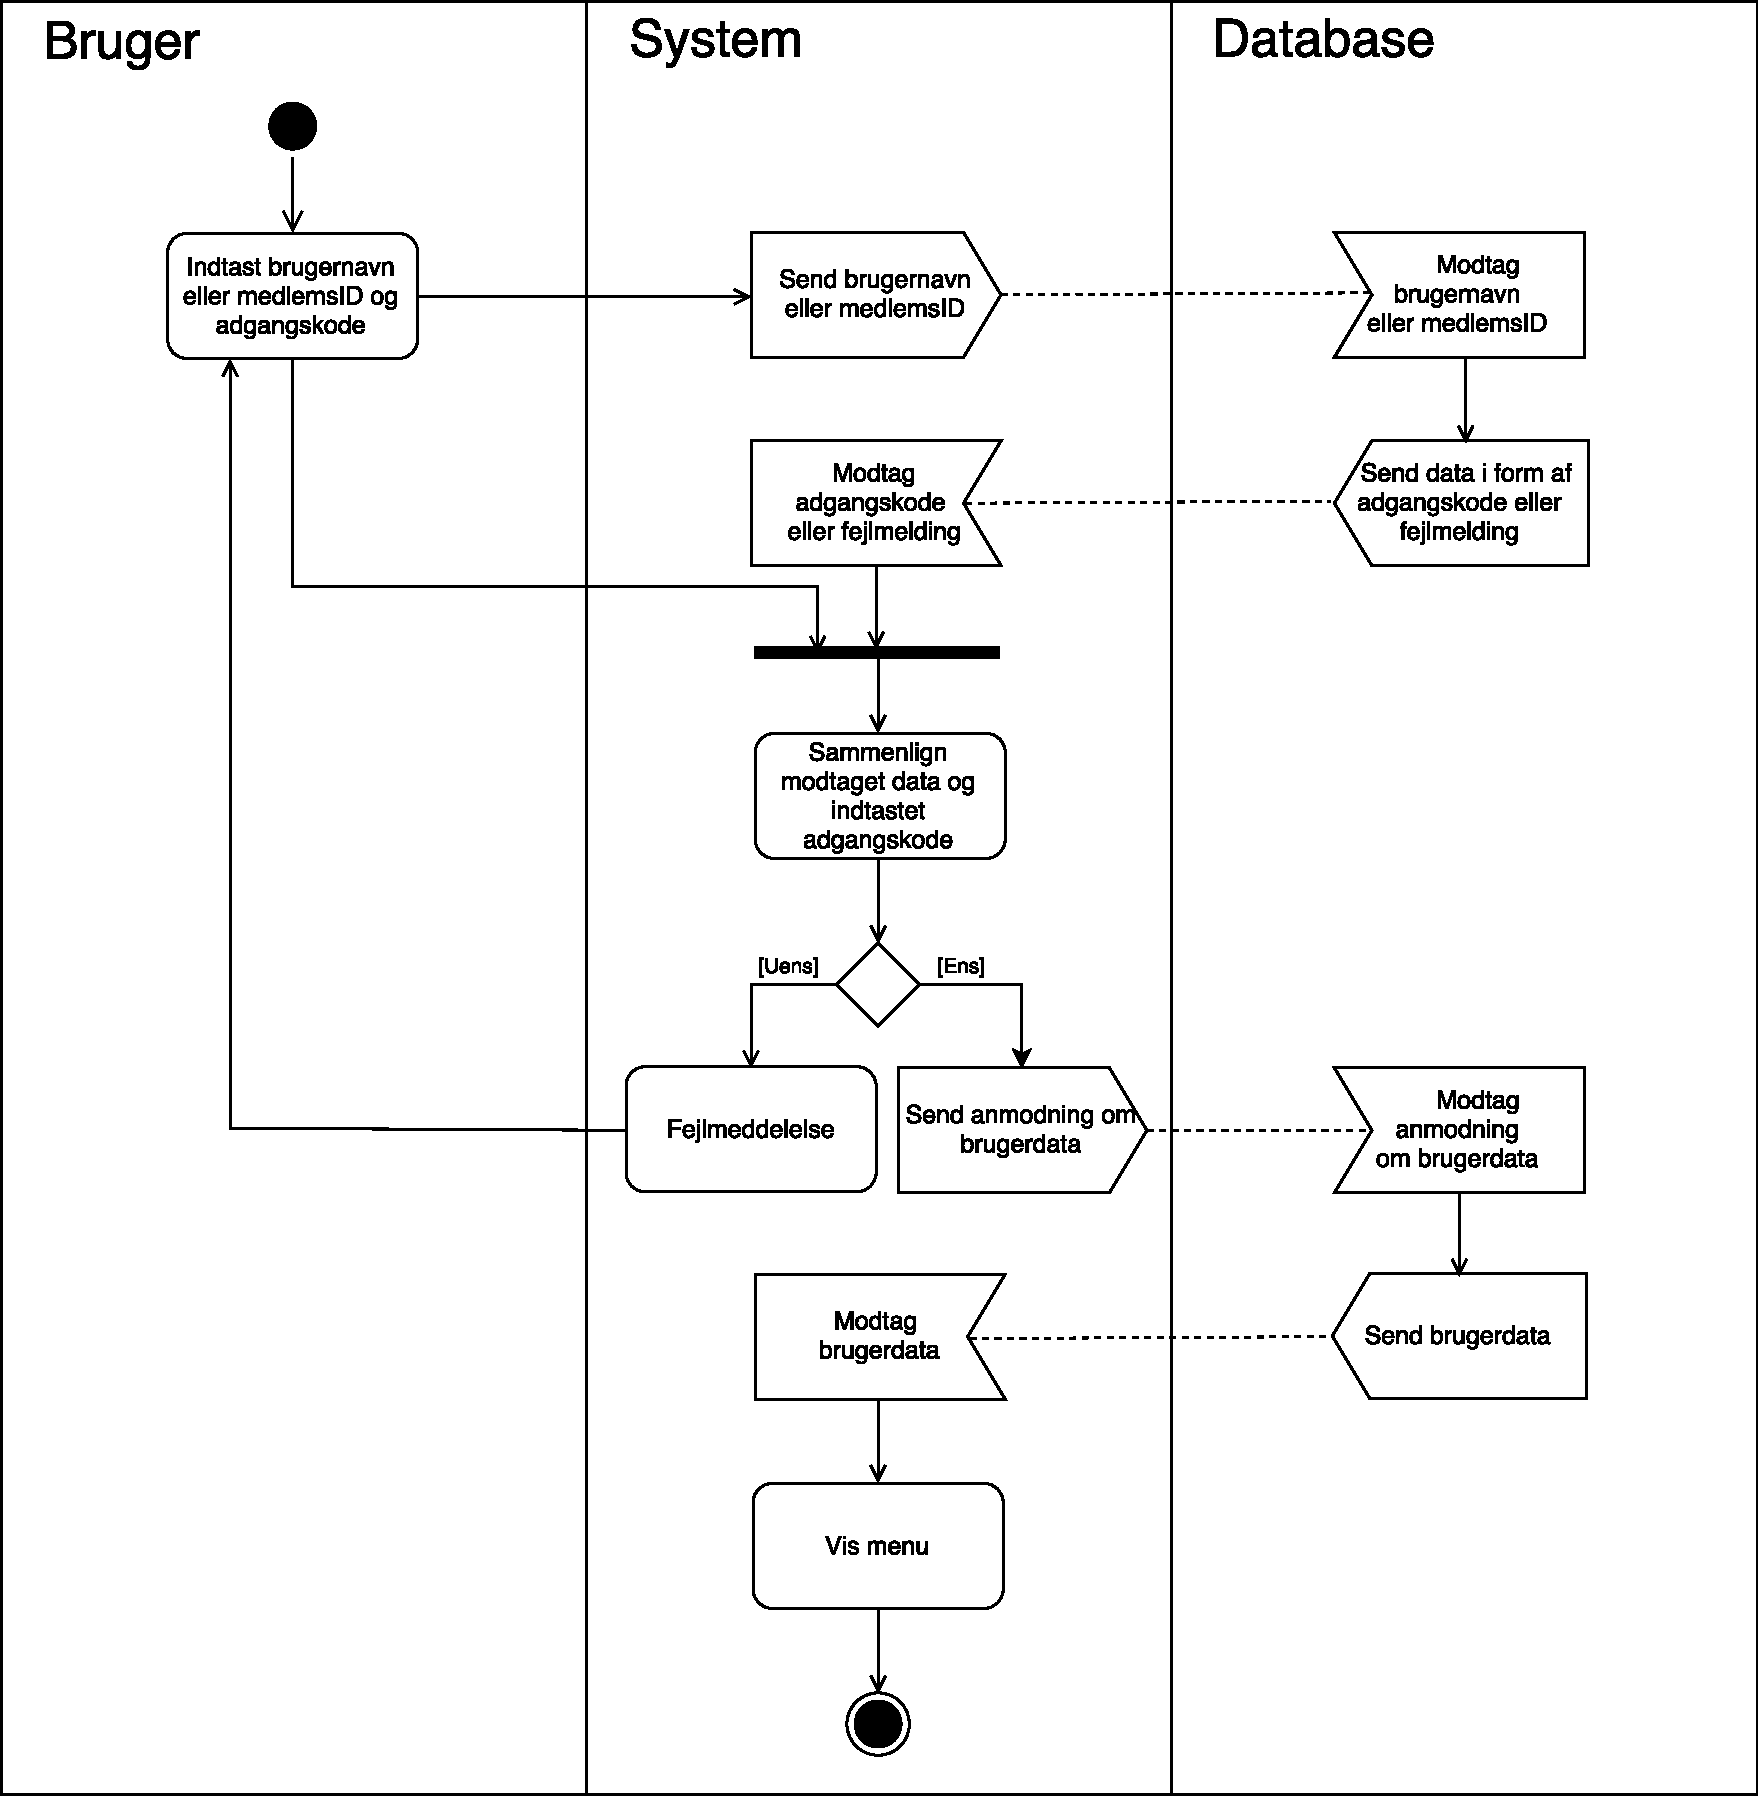
\includegraphics[width=0.9\textwidth]{figures/aktivitetsdiagram/Logind}
\caption{Aktivitetsdiagram over log ind.}
\label{fig:Logind}
\end{figure}

I figur \autoref{fig:logind} er aktivitetsdiagrammet over processen ved log ind illustreret. Når brugeren åbner app'en er der mulighed for at indtaste medlemsID eller brugernavn samt kodeord. Systemet sender det indtastede medlemsID eller brugernavn til databasen, som tilbagesender det tilhørende kodeord, hvis det findes i databasen. Er medlemsID'et eller brugernavnet ikke registreret i databasen, tilbagesender databasen en fejlmeddelelse, hvorefter brugeren har mulighed for at indtaste logininformationer igen. Returnerer databasen et tilhørende kodeord, sammenligner systemet dette kodeord med brugerens indtastede kodeord. Er de to kodeord ens, sender databasen brugerdata og viser app'ens startmenu, ellers viser systemet en fejlmeddelelse, og brugeren får mulighed for at indtaste logininformationer igen. (?????)


